% ====================================================
%  AI 基础设施接口互联研究 — 汇报 PPT
%  Author: 葛良晨
%  Date: 2026-05-25
%  Compile: latexmk -xelatex -shell-escape
% ====================================================
\documentclass[aspectratio=169, 10pt, UTF8]{ctexbeamer}

% ---------- 主题与颜色 ----------
\usetheme{Madrid}
\usecolortheme{default}

\definecolor{ieeeBlue}{RGB}{0, 83, 159}
\definecolor{ieeeRed}{RGB}{198, 38, 46}
\definecolor{ieeeGreen}{RGB}{0, 114, 41}
\definecolor{ieeeOrange}{RGB}{235, 110, 31}
\definecolor{darkGray}{RGB}{66, 66, 66}
\definecolor{gold}{RGB}{200, 150, 0}
\definecolor{darkblue}{RGB}{0, 0, 139}
\definecolor{darkred}{RGB}{180, 0, 0}
\definecolor{darkgreen}{RGB}{0, 128, 0}

\setbeamercolor{structure}{fg=ieeeBlue}
\setbeamercolor{alerted text}{fg=ieeeRed}
\setbeamercolor{example text}{fg=ieeeGreen}
\setbeamercolor{frametitle}{bg=ieeeBlue!15, fg=ieeeBlue}
\setbeamercolor{block title}{bg=ieeeBlue!15, fg=ieeeBlue}
\setbeamercolor{block body}{bg=ieeeBlue!5}
\setbeamercolor{block title example}{bg=ieeeGreen!15, fg=ieeeGreen}
\setbeamercolor{block body example}{bg=ieeeGreen!5}
\setbeamercolor{block title alerted}{bg=ieeeRed!15, fg=ieeeRed}
\setbeamercolor{block body alerted}{bg=ieeeRed!5}

% ---------- 包 ----------
\usepackage{graphicx}
\usepackage{booktabs}
\usepackage{tabularx}
\usepackage{multirow}
\usepackage[table]{xcolor}
\usepackage{amsmath,amssymb}
\usepackage{tikz}
\usetikzlibrary{positioning, calc, shapes.geometric, arrows.meta, backgrounds, fit, shadows}
\usepackage{hyperref}
\usepackage{listings}

% ---------- 页脚 ----------
\setbeamertemplate{footline}[frame number]

% ---------- 每节前显示目录 ----------
\AtBeginSection[]{
  \begin{frame}{本节内容}
    \tableofcontents[currentsection]
  \end{frame}
}

% ---------- 元信息 ----------
\title[AI 接口互联调研]{破局``内存墙''与``互联墙''：\\ AI 基础设施接口互联深度调研}
\subtitle{痛点分析 · 行业标杆 · 标准演进 · 创业方向}
\author[葛良晨]{葛良晨}
\institute[]{组会汇报 · AI 基础设施分析}
\date{2026年5月25日}

% ---------- 全局 TikZ 样式（在 frame 外定义，避免 beamer # 处理问题）----------
\tikzset{
  painboxR/.style={rectangle, draw=ieeeRed, fill=ieeeRed!8, thick,
                   minimum width=5.5cm, minimum height=2.5cm,
                   align=center, rounded corners=6pt, font=\normalsize},
  painboxB/.style={rectangle, draw=ieeeBlue, fill=ieeeBlue!8, thick,
                   minimum width=5.5cm, minimum height=2.5cm,
                   align=center, rounded corners=6pt, font=\normalsize},
  painboxO/.style={rectangle, draw=ieeeOrange, fill=ieeeOrange!8, thick,
                   minimum width=5.5cm, minimum height=2.5cm,
                   align=center, rounded corners=6pt, font=\normalsize},
  painboxG/.style={rectangle, draw=darkgreen, fill=darkgreen!8, thick,
                   minimum width=5.5cm, minimum height=2.5cm,
                   align=center, rounded corners=6pt, font=\normalsize},
  genboxG4/.style={rectangle, draw=gray, fill=gray!10, thick,
                   minimum width=2.8cm, minimum height=1.2cm,
                   align=center, rounded corners=3pt, font=\small},
  genboxG5/.style={rectangle, draw=darkblue, fill=darkblue!10, thick,
                   minimum width=2.8cm, minimum height=1.2cm,
                   align=center, rounded corners=3pt, font=\small},
  genboxG6/.style={rectangle, draw=ieeeBlue, fill=ieeeBlue!10, thick,
                   minimum width=2.8cm, minimum height=1.2cm,
                   align=center, rounded corners=3pt, font=\small},
  genboxG7/.style={rectangle, draw=ieeeRed, fill=ieeeRed!10, thick,
                   minimum width=2.8cm, minimum height=1.2cm,
                   align=center, rounded corners=3pt, font=\small},
  dirR/.style={rectangle, draw=ieeeRed, fill=ieeeRed!10, thick,
               minimum width=3.8cm, minimum height=1.5cm,
               align=center, rounded corners=5pt, font=\small\bfseries},
  dirB/.style={rectangle, draw=ieeeBlue, fill=ieeeBlue!10, thick,
               minimum width=3.8cm, minimum height=1.5cm,
               align=center, rounded corners=5pt, font=\small\bfseries},
  dirG/.style={rectangle, draw=ieeeGreen, fill=ieeeGreen!10, thick,
               minimum width=3.8cm, minimum height=1.5cm,
               align=center, rounded corners=5pt, font=\small\bfseries},
  dirO/.style={rectangle, draw=ieeeOrange, fill=ieeeOrange!10, thick,
               minimum width=3.8cm, minimum height=1.5cm,
               align=center, rounded corners=5pt, font=\small\bfseries},
  dirDB/.style={rectangle, draw=darkblue, fill=darkblue!10, thick,
               minimum width=3.8cm, minimum height=1.5cm,
               align=center, rounded corners=5pt, font=\small\bfseries},
}

\begin{document}

% ============================================
%  标题页
% ============================================
\begin{frame}
  \titlepage
\end{frame}

% ============================================
%  目录
% ============================================
\begin{frame}{汇报大纲}
  \tableofcontents
\end{frame}

% ================================================================
\section{背景：AI 基础设施的系统性危机}
% ================================================================

\begin{frame}{算力与数据传输的剪刀差}
  \centering
  \begin{tikzpicture}[
    scale=0.75,
    axis/.style={->, >=Stealth, thick},
    curveUp/.style={ieeeRed, very thick},
    curveDown/.style={ieeeBlue, very thick},
    mylabel/.style={font=\footnotesize},
  ]
    % Axes
    \draw[axis] (0,0) -- (10,0) node[right] {时间};
    \draw[axis] (0,0) -- (0,7) node[above] {相对增长};

    % Grid
    \foreach \y in {1,...,6} {
      \draw[gray!30] (0,\y) -- (10,\y);
    }
    \foreach \x in {1,...,9} {
      \draw[gray!30] (\x,0) -- (\x,7);
    }

    % Curves
    \draw[curveUp] (0,0.5) to[out=30,in=200] (3,1.2) to[out=20,in=190] (5,2.5)
                    to[out=10,in=185] (7,4.2) to[out=5,in=180] (9,6.5)
                    node[above, font=\normalsize\bfseries] {峰值算力 (FLOPS)};

    \draw[curveDown] (0,0.5) to[out=30,in=200] (3,0.9) to[out=20,in=190] (5,1.6)
                     to[out=10,in=185] (7,2.5) to[out=5,in=180] (9,3.8)
                     node[above, font=\normalsize\bfseries] {内存带宽 / 互联速率};

    % Gap annotation
    \draw[<->, ieeeOrange, ultra thick] (9,3.9) -- (9,6.4)
          node[midway, right, font=\small\bfseries, text=ieeeRed] {``互联墙''};
  \end{tikzpicture}

  \begin{alertblock}{核心矛盾}
    算力持续狂飙，但内存带宽与互联速率的增长远远落后 ——\\
    瓶颈正从\textbf{``计算受限''}向\textbf{``内存受限'' \& ``通信受限''}不可逆转地转移。
  \end{alertblock}
\end{frame}

\begin{frame}{四大核心痛点}
  \centering
  \begin{tikzpicture}[scale=0.62]
    \node[painboxR] (P1) at (0,0) {
      \textbf{\LARGE 1}\\[4pt]
      \textbf{``内存墙''危机}\\[6pt]
      HBM 产能售罄，KVCache 膨胀\\
      CPU 内存通道物理上限\\
      RDMA 延迟过高
    };

    \node[painboxB] (P2) at (7,0) {
      \textbf{\LARGE 2}\\[4pt]
      \textbf{封装与 Reticle 极限}\\[6pt]
      掩膜版天花板 $\to$ Chiplet\\
      3D 堆叠良率 $\sim$60\%\\
      散热极限 $\to$ 液冷
    };

    \node[painboxO] (P3) at (0,-3.5) {
      \textbf{\LARGE 3}\\[4pt]
      \textbf{信号完整性崩塌}\\[6pt]
      PCIe 6.0: 64\,GT/s PAM4\\
      PCIe 7.0: 128\,GT/s\\
      通道损耗 $<$32\,dB $\to$ 铜线几英寸即畸变
    };

    \node[painboxG] (P4) at (7,-3.5) {
      \textbf{\LARGE 4}\\[4pt]
      \textbf{封闭协议 + MoE 困境}\\[6pt]
      NVLink 生态锁定\\
      MoE 多播长尾延迟 $\sim$10ms\\
      ``吵闹邻居''效应
    };
  \end{tikzpicture}
\end{frame}

% ================================================================
\section{痛点深度分析}
% ================================================================

\begin{frame}{痛点 1：``内存墙''与 KVCache 瓶颈}
  \begin{columns}[T]
    \begin{column}{0.50\textwidth}
      \begin{block}{现状}
        \begin{itemize}
          \item LLM 长上下文 $\to$ KVCache 指数增长
          \item 单卡 HBM 容量有限（H100: 80\,GB, H200: 141\,GB）
          \item SK Hynix 2026 年\textbf{全部 HBM 产能已售罄}
          \item CoWoS 封装产能极度紧张
        \end{itemize}
      \end{block}
    \end{column}
    \begin{column}{0.50\textwidth}
      \begin{alertblock}{后果}
        \begin{itemize}
          \item 内存价格飙升，推高 TCO
          \item CPU DRAM 扩展受限于通道数
          \item RDMA 方案延迟过高 $\to$ GPU 闲置
          \item TTFT 无法满足推理 SLA
        \end{itemize}
      \end{alertblock}
    \end{column}
  \end{columns}

  \vspace{10pt}
  \centering
  \begin{tikzpicture}[
    scale=0.65,
    bar/.style={thick, minimum height=0.6cm, font=\small\bfseries},
  ]
    \node[font=\small] at (0,1.2) {需求增长};
    \node[font=\small] at (6.5,1.2) {供给增长};
    % KVCache demand
    \node[right] at (-3.5,0.6) {KVCache 需求};
    \draw[bar, ieeeRed, fill=ieeeRed!20] (0,0.6) -- (9.5,0.6);
    % HBM supply
    \node[right] at (-3.5,-0.6) {HBM 产能};
    \draw[bar, ieeeBlue, fill=ieeeBlue!20] (0,-0.6) -- (3.2,-0.6);
    % Memory bandwidth
    \node[right] at (-3.5,-1.8) {内存带宽};
    \draw[bar, ieeeGreen, fill=ieeeGreen!20] (0,-1.8) -- (4.0,-1.8);
    \draw[dashed, ieeeRed, ultra thick] (3.2,-2.3) -- (3.2,1.2)
          node[above, font=\small] {剪刀差};
  \end{tikzpicture}
\end{frame}

\begin{frame}{痛点 2：Reticle 极限与 Chiplet 转型}
  \centering
  \begin{tikzpicture}[
    scale=0.6,
    chip/.style={rectangle, draw=ieeeBlue, thick, minimum width=3cm,
                 minimum height=3cm, rounded corners=4pt, fill=ieeeBlue!5},
    chiplet/.style={rectangle, draw=ieeeRed, thick, minimum width=1.3cm,
                    minimum height=1.3cm, rounded corners=2pt, fill=ieeeRed!8,
                    align=center},
    d2d/.style={<->, >=Stealth, very thick, ieeeOrange},
    mylabel/.style={font=\footnotesize\bfseries},
  ]
    % Monolithic era
    \node[mylabel, ieeeBlue] (MONO_T) at (0,4) {过去的单体芯片};
    \node[chip] (MONO) at (0,1.8) {};
    \node[font=\footnotesize] at (0,2.5) {单一 Die};
    \node[font=\footnotesize] at (0,1.5) {$\sim$800\,mm\textsuperscript{2}};
    \node[font=\footnotesize] at (0,0.8) {已达极限};
    \draw[ieeeRed, very thick] (-1.5,0.3) -- (1.5,3.3);
    \node[font=\small\bfseries, ieeeRed, align=center] at (2.2,1.8) {Reticle\\Limit};

    % Arrow
    \draw[->, >=Stealth, ultra thick, darkGray] (3.5,1.8) -- (5.5,1.8)
          node[midway, above, font=\small] {转型};

    % Chiplet era
    \node[mylabel, ieeeRed] (CHIP_T) at (9,4) {现在与未来：Chiplet 架构};
    \draw[rounded corners=6pt, ieeeBlue, thick, fill=ieeeBlue!3]
         (7,0.3) rectangle (11,3.3);
    \node[chiplet] (C1) at (8.2,2.5) {Compute\\Die};
    \node[chiplet] (C2) at (9.8,2.5) {Compute\\Die};
    \node[chiplet, fill=ieeeGreen!10] (C3) at (8.2,0.8) {I/O\\Die};
    \node[chiplet, fill=ieeeOrange!10] (C4) at (9.8,0.8) {HBM\\Die};
    \draw[d2d] (C1) -- (C2);
    \draw[d2d] (C1) -- (C3);
    \draw[d2d] (C2) -- (C4);
    \draw[d2d] (C3) -- (C4);

    % Issues
    \node[font=\footnotesize, below=0.3cm of C4, align=center, text=ieeeRed]
         {3D 堆叠良率 $\sim$60\%\\散热 $\to$ 液冷};
  \end{tikzpicture}
\end{frame}

\begin{frame}{痛点 3：高速信号物理极限}
  \centering
  \begin{tikzpicture}[
    scale=0.55,
    arrow/.style={->, >=Stealth, thick},
  ]
    % PCIe generations
    \node[genboxG4] (G4)  at (0,0)    {PCIe 4.0\\16\,GT/s\\NRZ};
    \node[genboxG5] (G5)  at (4,0)    {PCIe 5.0\\32\,GT/s\\NRZ};
    \node[genboxG6] (G6)  at (8,0)    {PCIe 6.0\\64\,GT/s\\\textbf{PAM4}};
    \node[genboxG7] (G7)  at (12,0)   {PCIe 7.0\\128\,GT/s\\\textbf{PAM4}};

    \draw[arrow] (G4) -- (G5);
    \draw[arrow] (G5) -- (G6);
    \draw[arrow] (G6) -- (G7);

    % Channel loss limits
    \node[font=\footnotesize, below=0.3cm of G4, text=gray]
         {损耗: 28\,dB};
    \node[font=\footnotesize, below=0.3cm of G5, text=darkblue]
         {损耗: 36\,dB};
    \node[font=\footnotesize, below=0.3cm of G6, text=ieeeBlue]
         {损耗: 32\,dB（更严苛）};
    \node[font=\footnotesize, below=0.3cm of G7, text=ieeeRed]
         {损耗: $<$32\,dB};

    % PAM4 explanation
    \begin{scope}[yshift=-3cm]
      \node[font=\normalsize\bfseries] at (3,0) {NRZ (PAM2)};
      \node[font=\normalsize\bfseries] at (9,0) {PAM4};

      \draw[->, >=Stealth] (0,-1.5) -- (6,-1.5) node[right] {2 电平 $\to$ 1 bit/symbol};
      \draw[->, >=Stealth] (6.5,-1.5) -- (12,-1.5) node[right] {4 电平 $\to$ 2 bit/symbol};

      \draw[ieeeBlue, ultra thick] (0,0.3) -- (1.5,0.3) -- (2.5,2.2) -- (4.5,2.2) -- (6,0.3);
      \draw[ieeeRed, ultra thick] (7,0.3) -- (7.8,0.3) -- (8.8,1.4) -- (9.6,2.8) -- (10.5,2.2) -- (11.5,0.8);

      \node[font=\small, text=ieeeRed, font=\bfseries] at (9,-0.5)
           {噪声敏感度 $\uparrow$ 眼图闭合 $\uparrow$};
    \end{scope}
  \end{tikzpicture}

  \begin{alertblock}{关键结论}
    PAM4 + 128\,GT/s $\to$ 传统铜线 \textbf{几英寸内严重畸变} $\to$ 必须引入 Retimer / 光互联
  \end{alertblock}
\end{frame}

\begin{frame}{痛点 4：MoE 路由困境与``吵闹邻居''}
  \begin{columns}[T]
    \begin{column}{0.48\textwidth}
      \begin{block}{MoE 多播挑战}
        \begin{itemize}
          \item 256 专家中激活 8 个，分布在不同 GPU
          \item 交换机多播配置长尾延迟 $\sim$10\,ms
          \item 训练时被迫限制专家分布 $\leq$4 节点
          \item \textbf{硬件妥协 $\to$ 模型能力受损}
        \end{itemize}
      \end{block}
    \end{column}
    \begin{column}{0.48\textwidth}
      \begin{alertblock}{Noisy Neighbor}
        \begin{itemize}
          \item GPU/NIC/SSD 共享 PCIe 交换核心
          \item SSD I/O 抢占仲裁 $\to$ GPU 流阻塞
          \item 不可预测的延迟抖动
          \item \textbf{AI 集群效率严重下降}
        \end{itemize}
      \end{alertblock}
    \end{column}
  \end{columns}

  \vspace{8pt}
  \centering
  \begin{tikzpicture}[
    scale=0.55,
    nodebox/.style={rectangle, draw=ieeeBlue, thick, minimum width=1.5cm,
                    minimum height=0.8cm, rounded corners=3pt, align=center,
                    font=\footnotesize},
    arrow/.style={->, >=Stealth, thick, ieeeRed},
  ]
    \node[nodebox, fill=ieeeRed!10] (GPU) {GPU};
    \node[nodebox, fill=ieeeBlue!10, right=of GPU] (SW) {Shared\\Switch};
    \node[nodebox, fill=ieeeGreen!10, above right=of SW] (NIC) {NIC};
    \node[nodebox, fill=ieeeOrange!10, below right=of SW] (SSD) {SSD};

    \draw[arrow] (GPU) -- (SW);
    \draw[arrow] (SW) -- (NIC);
    \draw[arrow, ultra thick, ieeeRed] (SSD) -- (SW)
          node[midway, below, font=\tiny, text=ieeeRed] {抢占仲裁};

    \node[font=\small\bfseries, text=ieeeRed, below=1.5cm of SW]
         {共享核心 $\to$ 流量相互阻塞};
  \end{tikzpicture}
\end{frame}

% ================================================================
\section{行业标杆：Astera Labs 与前沿企业}
% ================================================================

\begin{frame}{Astera Labs 产品矩阵总览}
  \centering
  \begin{tikzpicture}[
    scale=0.55,
    product/.style={rectangle, draw=ieeeBlue, fill=ieeeBlue!8, thick,
                    minimum width=4cm, minimum height=1.5cm,
                    align=center, rounded corners=4pt, font=\normalsize},
    arrow/.style={->, >=Stealth, thick, ieeeBlue},
  ]
    \node[font=\LARGE\bfseries, ieeeBlue] at (0,3.5)
         {``Purpose-Built Connectivity for Rack-Scale AI''};

    % Physical layer
    \node[product, fill=ieeeRed!8] (ARIES) at (-5,0)
         {\textbf{Aries 系列}\\PCIe/CXL Retimer \& Smart Cable};
    \node[product, fill=ieeeOrange!8] (TAURUS) at (5,0)
         {\textbf{Taurus 系列}\\Ethernet Smart Cable Module (800G)};

    % Switch layer
    \node[product, fill=gold!12] (SCORPIO) at (0,-2.5)
         {\textbf{Scorpio 系列}\\Smart Fabric Switch (32--320 Lanes)};

    % Memory layer
    \node[product, fill=ieeeGreen!8] (LEO) at (0,-5)
         {\textbf{Leo 系列}\\CXL Smart Memory Controller (2\,TB)};

    % Software
    \node[product, fill=gray!10] (COSMOS) at (0,-7.5)
         {\textbf{COSMOS}\\Telemetry \& Fleet Management};

    \draw[arrow] (ARIES.south) -- (SCORPIO.north west);
    \draw[arrow] (TAURUS.south) -- (SCORPIO.north east);
    \draw[arrow] (SCORPIO.south) -- (LEO.north);
    \draw[arrow] (LEO.south) -- (COSMOS.north);

    \node[font=\footnotesize, right=0.5cm of ARIES, text=ieeeRed]
         {物理层：信号延展};
    \node[font=\footnotesize, right=0.5cm of SCORPIO, text=gold]
         {架构层：智能交换};
    \node[font=\footnotesize, right=0.5cm of COSMOS, text=darkGray]
         {系统层：管理运维};
  \end{tikzpicture}
\end{frame}

\begin{frame}{物理层：Aries Retimer \& Smart Cable}
  \begin{columns}[T]
    \begin{column}{0.50\textwidth}
      \begin{block}{Aries DSP Retimer}
        \begin{itemize}
          \item 64\,GT/s PAM4 SerDes
          \item 信号传输距离 \textbf{可靠延长 3$\times$}
          \item 填补 32\,dB 损耗预算鸿沟
          \item 小型封装，集成 AC 耦合电容
        \end{itemize}
      \end{block}
    \end{column}
    \begin{column}{0.50\textwidth}
      \begin{exampleblock}{Aries Smart Cable Module}
        \begin{itemize}
          \item 有源电缆 (AEC) 技术
          \item 密集 AI 机架内部署 PCIe/CXL
          \item 释放跨机架 GPU-GPU 拓扑
          \item 灵活时钟模式
        \end{itemize}
      \end{exampleblock}
    \end{column}
  \end{columns}

  \vspace{10pt}
  \centering
  \begin{tikzpicture}[
    scale=0.55,
    box/.style={rectangle, draw=ieeeBlue, thick, minimum width=2cm,
                minimum height=0.8cm, rounded corners=3pt, align=center,
                font=\small},
    arrow/.style={->, >=Stealth, ultra thick},
  ]
    \node[box, fill=ieeeRed!5] (CPU) {CPU};
    \node[box, fill=ieeeBlue!5, right=2cm of CPU] (RET) {Aries\\Retimer};
    \node[box, fill=ieeeRed!5, right=2cm of RET] (GPU) {GPU};

    \draw[arrow, ieeeRed] (CPU) -- node[above, font=\small, text=ieeeRed]
         {信号衰减} (RET);
    \draw[arrow, ieeeGreen] (RET) -- node[above, font=\small, text=ieeeGreen]
         {信号重建} (GPU);

    \node[font=\footnotesize, below=0.5cm of RET]
         {DSP 均衡 + 时钟恢复 $\to$ 延展 3$\times$};
  \end{tikzpicture}
\end{frame}

\begin{frame}{物理层：Taurus 以太网智能线缆}
  \begin{columns}[T]
    \begin{column}{0.55\textwidth}
      \begin{itemize}
        \item 支持 \textbf{800G}（100G/Lane PAM4）以太网
        \item 极细铜缆（30/32/34 AWG）$\to$ 3\,m 可靠连接
        \item 弯曲半径减半 $\to$ 优化散热气流
        \item 内置 PRBS 发生器/检查器
        \item 实时温度、电压\textbf{遥测}
        \item 安全固件无线更新（OTA）
      \end{itemize}
    \end{column}
    \begin{column}{0.45\textwidth}
      \begin{alertblock}{对比传统方案}
        \begin{itemize}
          \item 替代粗重无源铜缆
          \item 替代昂贵有源光缆（部分场景）
          \item 大幅简化机架布线
          \item ToR 到 NIC 连接首选
        \end{itemize}
      \end{alertblock}
    \end{column}
  \end{columns}
\end{frame}

\begin{frame}{内存层：Leo CXL 智能内存控制器}
  \begin{columns}[T]
    \begin{column}{0.50\textwidth}
      \begin{block}{Leo 核心能力}
        \begin{itemize}
          \item CXL 2.0 协议，支持内存扩展 \& 池化
          \item 单控制器 \textbf{2\,TB 容量扩展}
          \item 服务器内存容量 $\uparrow$ 1.5$\times$+
          \item 端到端数据完整性保护
          \item 服务器级 RAS 定制化
        \end{itemize}
      \end{block}
    \end{column}
    \begin{column}{0.50\textwidth}
      \begin{exampleblock}{软件协同：MemVerge}
        \begin{itemize}
          \item \textbf{Elastic Memory}：动态按需分配 CXL 池内存
          \item 实时监控内存热力图
          \item 消除 OOM 崩溃
          \item 解决``内存搁浅''问题
          \item \textbf{Gismo}：零 IO 共享内存对象
        \end{itemize}
      \end{exampleblock}
    \end{column}
  \end{columns}

  \vspace{8pt}
  \centering
  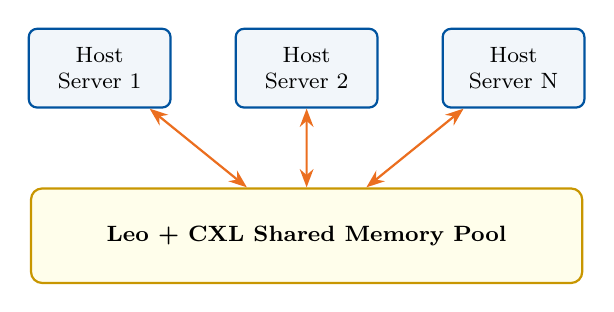
\begin{tikzpicture}[
    scale=0.55,
    server/.style={rectangle, draw=ieeeBlue, thick, minimum width=1.8cm,
                   minimum height=1cm, rounded corners=3pt, align=center,
                   fill=ieeeBlue!5, font=\footnotesize},
    arrow/.style={<->, >=Stealth, thick, ieeeOrange},
  ]
    \node[server] (S1) {Host\\Server 1};
    \node[server, right=0.8cm of S1] (S2) {Host\\Server 2};
    \node[server, right=0.8cm of S2] (S3) {Host\\Server N};

    \node[rectangle, draw=gold, fill=yellow!8, thick,
          minimum width=7cm, minimum height=1.2cm, align=center,
          rounded corners=4pt, font=\footnotesize\bfseries,
          below=1cm of S2] (POOL) {Leo + CXL Shared Memory Pool};

    \draw[arrow] (S1) -- (POOL);
    \draw[arrow] (S2) -- (POOL);
    \draw[arrow] (S3) -- (POOL);
  \end{tikzpicture}
\end{frame}

\begin{frame}{交换层：Scorpio Smart Fabric Switch}
  \begin{block}{P 系列：硬件隔离消除 Noisy Neighbor}
    \begin{itemize}
      \item 32--320 通道全矩阵配置
      \item GPU/CPU/NIC ``连接岛'' 与 SSD ``连接岛'' \textbf{物理隔离}
      \item 独立交换核心 + 独立仲裁逻辑 $\to$ 零性能损耗
    \end{itemize}
  \end{block}

  \begin{exampleblock}{X 系列：硬件加速破解 MoE 瓶颈}
    \begin{itemize}
      \item 320 通道 + \textbf{Hypercast} 硬件多播引擎
      \item \textbf{In-Network Compute}：交换机内直接聚合
      \item AI 集合操作效率 $\uparrow$ 2$\times$，单跳连接 80 加速器
      \item 直接内存语义通信，绕过 CPU 协议栈
    \end{itemize}
  \end{exampleblock}

  \begin{alertblock}{安全}
    Secure Boot + 不可变硬件信任根 (RoT) $\to$ 全链路防篡改 + COSMOS 遥测
  \end{alertblock}
\end{frame}

\begin{frame}{混合网络架构：Marvell \& XConn}
  \begin{columns}[T]
    \begin{column}{0.52\textwidth}
      \begin{block}{Marvell 收购 XConn（\$5.4 亿）}
        \begin{itemize}
          \item \textbf{Apollo 2}：业界首款混合交换芯片
          \item 单硅片同时处理：
          \begin{itemize}
            \item CXL 3.1
            \item PCIe Gen 6.2
          \end{itemize}
          \item \textbf{Structera S} 系列：260 通道
          \item 消除多级级联
        \end{itemize}
      \end{block}
    \end{column}
    \begin{column}{0.48\textwidth}
      \begin{alertblock}{战略意图}
        \begin{itemize}
          \item 统一开放 Fabric 平台
          \item 目标：挑战 NVIDIA NVLink 垄断
          \item 不绑定单一协议生态
        \end{itemize}
      \end{alertblock}

      \vspace{10pt}
      \begin{center}
        \textbf{混合交换 $\to$ 统一互联的终局形态}
      \end{center}
    \end{column}
  \end{columns}
\end{frame}

\begin{frame}{Enfabrica：超级网卡 (SuperNIC) 新范式}
  \begin{columns}[T]
    \begin{column}{0.50\textwidth}
      \begin{block}{ACF-S Millennium 芯片}
        \begin{itemize}
          \item \textbf{3.2\,Tbps} 吞吐量 SuperNIC
          \item 多端口 800G 以太网
          \item 32 端口多路径喷射
          \item 4$\times$ 传统网卡带宽
        \end{itemize}
      \end{block}
    \end{column}
    \begin{column}{0.50\textwidth}
      \begin{exampleblock}{技术亮点}
        \begin{itemize}
          \item Multi-path Spraying：\textbf{非点对点、多路径冗余}
          \item 网络阻塞时无缝负载均衡
          \item 极度容错的并发数据通道
          \item 已获 \$1.15 亿 C 轮融资
        \end{itemize}
      \end{exampleblock}
    \end{column}
  \end{columns}

  \vspace{8pt}
  \centering
  \begin{tikzpicture}[
    scale=0.55,
    nodebox/.style={rectangle, draw=ieeeBlue, thick, minimum width=1.5cm,
                    minimum height=0.8cm, rounded corners=3pt, align=center,
                    font=\footnotesize},
    arrow/.style={->, >=Stealth, thick},
  ]
    \node[nodebox, fill=ieeeRed!8] (SRC) {Source};
    \node[nodebox, fill=ieeeGreen!8, right=1.5cm of SRC] (NIC) {ACF-S\\SuperNIC};
    \node[nodebox, fill=ieeeBlue!8, above right=1.2cm of NIC] (P1) {Path 1};
    \node[nodebox, fill=ieeeBlue!8, right=1.2cm of NIC] (P2) {Path 2};
    \node[nodebox, fill=ieeeBlue!8, below right=1.2cm of NIC] (P3) {Path 3};

    \draw[arrow] (SRC) -- (NIC);
    \draw[arrow] (NIC) -- (P1);
    \draw[arrow] (NIC) -- (P2);
    \draw[arrow] (NIC) -- (P3);

    \node[font=\small\bfseries, below=1.5cm of NIC, text=ieeeOrange]
         {32 路径并发喷射 $\to$ 任意路径容错};
  \end{tikzpicture}
\end{frame}

\begin{frame}{Eliyan：标准封装下的高性能 Die-to-Die}
  \centering
  \begin{tikzpicture}[
    scale=0.55,
    pkg/.style={rectangle, draw=gray, thick, minimum width=5cm,
                minimum height=3cm, rounded corners=4pt, fill=gray!5},
    die/.style={rectangle, draw=ieeeBlue, thick, minimum width=1.3cm,
                minimum height=1.3cm, rounded corners=2pt, fill=ieeeBlue!8},
    d2d/.style={<->, >=Stealth, ultra thick, ieeeRed},
  ]
    % Advanced packaging
    \node[font=\normalsize\bfseries] at (-2.5,3) {先进封装 (CoWoS)};
    \node[pkg, fill=ieeeRed!5] at (-2.5,0) {};
    \node[font=\footnotesize, align=center] at (-2.5,-1.8)
         {硅中介层\\40--55\,\textmu m 凸点间距\\成本极高、产能紧缺};

    \node[die] (AD1) at (-3.3,0.5) {Die A};
    \node[die] (AD2) at (-1.7,0.5) {Die B};
    \draw[d2d, ieeeOrange] (AD1) -- (AD2);

    % Arrow
    \draw[->, >=Stealth, ultra thick, darkGray] (1,0) -- (3,0);

    % Standard packaging
    \node[font=\normalsize\bfseries] at (7,3) {Eliyan NuLink 方案};
    \node[pkg, fill=ieeeGreen!5, minimum width=5.5cm, minimum height=3.5cm] at (7,0) {};
    \node[font=\footnotesize, align=center] at (7,-2.2)
         {标准有机基板\\100--130\,\textmu m 凸点间距\\成本低、供应链成熟};

    \node[die] (ED1) at (5.8,0.5) {Die A};
    \node[die] (ED2) at (8.2,0.5) {Die B};
    \draw[d2d, ieeeGreen] (ED1) -- (ED2)
          node[midway, above, font=\tiny\bfseries, text=ieeeRed]
               {224\,Gbps/lane!};

    \node[font=\small\bfseries, text=ieeeRed] at (7,1.5)
         {同等带宽 \& 延迟，成本大幅降低};
  \end{tikzpicture}

  \begin{itemize}
    \item NuLink PHY：高级均衡 + 信道调制，兼容 UCIe/BoW 开放标准
    \item 单向速率：64G $\to$ \textbf{224G}，研发 448G
  \end{itemize}
\end{frame}

\begin{frame}{终局形态：硅光与共封装光学 (CPO)}
  \centering
  \begin{tikzpicture}[
    scale=0.55,
    techbox/.style={rectangle, draw=ieeeBlue, fill=ieeeBlue!8, thick,
                    minimum width=3.5cm, minimum height=2.5cm,
                    align=center, rounded corners=5pt, font=\small},
  ]
    % Ayar Labs
    \node[techbox, fill=ieeeRed!8] (AYAR) at (-5.5,0) {
      \textbf{Ayar Labs}\\[4pt]
      TeraPHY 光学 I/O 芯粒\\
      CPO 架构：\textbf{8\,Tbps}\\
      5--10$\times$ 带宽 vs 铜\\
      4--8$\times$ 能效提升\\
      10$\times$ 延迟降低\\[2pt]
      \textit{\$5 亿 E 轮, 估值 \$37.5 亿}
    };

    % Celestial AI
    \node[techbox, fill=gold!10] (CEL) at (0,0) {
      \textbf{Celestial AI}\\[4pt]
      Photonic Fabric\\
      3D 垂直共封装\\
      不占硅片边缘面积\\
      释放 HBM 集成空间\\[2pt]
      \textit{Marvell \$32.5 亿收购}
    };

    % Avicena
    \node[techbox, fill=ieeeGreen!8] (AVI) at (5.5,0) {
      \textbf{Avicena}\\[4pt]
      GaN 微型 LED 阵列\\
      超低功耗短距光通信\\
      替代高速激光器\\
      高并发、低单路速率\\[2pt]
      \textit{10\,m 内互联新范式}
    };
  \end{tikzpicture}

  \vspace{12pt}
  \begin{center}
    \textbf{当铜互联触达物理极限 $\to$ 全光网络是唯一出路}
  \end{center}
\end{frame}

% ================================================================
\section{前沿互联标准演进}
% ================================================================

\begin{frame}{开放标准突围：UALink \& UEC}
  \begin{columns}[T]
    \begin{column}{0.48\textwidth}
      \begin{block}{UALink (Scale-Up)}
        \begin{itemize}
          \item \textbf{1.0} (2025)：单通道 200G/128G
          \item 单 Pod 直连 \textbf{1,024} 加速器
          \item 原生 Load/Store 内存语义
          \item \textbf{2.0} (2026 Q2)：引入 In-Network Compute
          \item 兼容 UCIe 3.0 Chiplet 标准
        \end{itemize}
      \end{block}
    \end{column}
    \begin{column}{0.48\textwidth}
      \begin{exampleblock}{UEC (Scale-Out)}
        \begin{itemize}
          \item \textbf{1.0} (2025)，1.0.2 (2026)
          \item 重构以太网协议栈
          \item 灵活拥塞管理 (CMS)
          \item 多路径并发喷射
          \item 微小报文性能极致优化
          \item $\to$ 接近无损网络性能
        \end{itemize}
      \end{exampleblock}
    \end{column}
  \end{columns}

  \begin{alertblock}{共同目标}
    打破 NVLink 等封闭协议垄断，建立\textbf{多厂商、开放、互操作}的 AI 互联标准
  \end{alertblock}
\end{frame}

\begin{frame}{PCIe 7.0 时代的测试验证挑战}
  \centering
  \begin{tikzpicture}[
    scale=0.55,
    testbox/.style={rectangle, draw=ieeeBlue, thick, minimum width=4.5cm,
                    minimum height=1.8cm, rounded corners=4pt, align=center,
                    fill=ieeeBlue!5, font=\footnotesize},
  ]
    \node[font=\LARGE\bfseries, ieeeRed] at (0,3) {128\,GT/s $\to$ 眼图完全闭合};

    \node[testbox] (K1) at (-3.5,0.5) {
      \textbf{Keysight}\\
      N5991PB7A 自动化接收器测试\\
      API 联动 M8050A BERT\\
      TP2/TP3 微秒级精准校准
    };

    \node[testbox] (K2) at (3.5,0.5) {
      \textbf{Viavi}\\
      Xgig PCIe 7.0 协议分析平台\\
      全栈协议解码 (PCIe/CXL/NVMe)\\
      LTSSM 强制覆盖测试
    };

    \node[testbox, fill=ieeeOrange!8] (K3) at (0,-2.5) {
      \textbf{关键变革}\\
      手动调示波器 $\to$ \textbf{AI 驱动自动化验证}\\
      传统线缆探测 $\to$ \textbf{超低损耗插入器}\\
      流片后测试 $\to$ \textbf{流片前数字孪生仿真}
    };
  \end{tikzpicture}

  \begin{center}
    测试验证是 PCIe 7.0 时代最容易被忽视的\textbf{隐形壁垒}
  \end{center}
\end{frame}

% ================================================================
\section{五大创业方向}
% ================================================================

\begin{frame}{创业方向全景图}
  \centering
  \begin{tikzpicture}[
    scale=0.55,
    mid/.style={rectangle, draw=ieeeBlue, fill=ieeeBlue!5, thick,
                minimum width=9cm, minimum height=1.2cm,
                align=center, rounded corners=6pt, font=\normalsize\bfseries},
  ]
    % Top: Center mission
    \node[mid, draw=ieeeRed, fill=ieeeRed!5] at (0,3)
         {破局``内存墙''与``互联墙''};

    \node[dirR] (D1) at (-6,0.5) {方向一\\CXL 推理存储\\中间件};

    \node[dirB] (D2) at (0,0.5) {方向二\\标准封装\\D2D PHY IP};

    \node[dirG] (D3) at (6,0.5) {方向三\\多协议融合\\SuperNIC};

    \node[dirO] (D4) at (-3,-2.5) {方向四\\硅光/CPO\\核心组件};

    \node[dirDB] (D5) at (3,-2.5) {方向五\\AI 驱动\\验证系统};

    % Connections
    \draw[->, >=Stealth, thick, ieeeBlue!50] (-2,2.5) -- (D1);
    \draw[->, >=Stealth, thick, ieeeBlue!50] (0,2.5) -- (D2);
    \draw[->, >=Stealth, thick, ieeeBlue!50] (2,2.5) -- (D3);
    \draw[->, >=Stealth, thick, ieeeBlue!50] (-2,2.5) -- (D4);
    \draw[->, >=Stealth, thick, ieeeBlue!50] (2,2.5) -- (D5);
  \end{tikzpicture}
\end{frame}

\begin{frame}{方向一：CXL 原生语义的推理存储中间件}
  \begin{block}{痛点}
    现有 Linux 内核未针对 CXL NUMA 优化，传统 RDMA 多级开销导致 KVCache 跨节点效率极低
  \end{block}

  \begin{columns}[T]
    \begin{column}{0.50\textwidth}
      \textbf{技术路线：}
      \begin{enumerate}
        \item \textbf{弹性内存服务}：内核级热力图监控 + 亚毫秒 CXL 映射 $\to$ 消除 OOM
        \item \textbf{原生 KVCache 底座}：基于 Beluga 架构，GPU 直接 Load/Store 远程 KVCache
        \item \textbf{Zero-IO 张量管理器}：CXL 共享内存消除网络拷贝
      \end{enumerate}
    \end{column}
    \begin{column}{0.50\textwidth}
      \begin{exampleblock}{核心指标}
        \begin{itemize}
          \item TTFT $\downarrow$ \textbf{89.6\%} (Beluga 实测)
          \item 吞吐量 $\uparrow$ \textbf{7.35$\times$}
          \item 完全旁路 CPU \& RDMA 协议栈
        \end{itemize}
      \end{exampleblock}

      \begin{alertblock}{商业价值}
        被云厂商收购的极高潜力
      \end{alertblock}
    \end{column}
  \end{columns}
\end{frame}

\begin{frame}{方向二：标准封装的 D2D 互联 IP}
  \begin{block}{痛点}
    CoWoS 先进封装成本极高、产能瓶颈严重 $\to$ AI 芯片出货受限
  \end{block}

  \vspace{6pt}
  \begin{columns}[T]
    \begin{column}{0.55\textwidth}
      \begin{itemize}
        \item 对标 Eliyan NuLink 技术
        \item 标准有机基板实现先进封装级 D2D 带宽
        \item 混合信号均衡 + 高级 FEC
        \item 64G PAM4 $\to$ 224G $\to$ 448G
        \item 兼容 \textbf{UCIe 3.0 \& BoW} 开放标准
      \end{itemize}
    \end{column}
    \begin{column}{0.45\textwidth}
      \begin{exampleblock}{附加高价值方向}
        \begin{itemize}
          \item Chiplet 内网硬件防火墙
          \item 基于 UCIe UDA 的异常检测 IP
          \item 防硬件木马窥探显存
        \end{itemize}
      \end{exampleblock}
    \end{column}
  \end{columns}

  \vspace{8pt}
  \begin{center}
    \textbf{即插即用的模块化 IP $\to$ 颠覆半导体制造成本结构}
  \end{center}
\end{frame}

\begin{frame}{方向三：多协议融合智能 SuperNIC}
  \begin{block}{痛点}
    AI 集群需同时处理以太网摄入 + UALink 纵向互联 + CXL 内存解构，现有 NIC 成瓶颈
  \end{block}

  \begin{columns}[T]
    \begin{column}{0.50\textwidth}
      \begin{block}{混合 Fabric 交换引擎}
        单硅片原生支持：
        \begin{itemize}
          \item 以太网 (UEC 标准)
          \item PCIe 6.0/7.0
          \item CXL 3.1
          \item UALink 1.0/2.0
        \end{itemize}
        对标：XConn Apollo 2
      \end{block}
    \end{column}
    \begin{column}{0.50\textwidth}
      \begin{exampleblock}{弹性 AI 通信 SuperNIC}
        \begin{itemize}
          \item 多端口 800G 超以太网
          \item 硬件卸载 AllReduce/AllGather 等集合通信
          \item 多路径容错 + 动态流量喷射
          \item 大幅降低尾随延迟
        \end{itemize}
        对标：Enfabrica ACF-S (3.2\,Tbps)
      \end{exampleblock}
    \end{column}
  \end{columns}
\end{frame}

\begin{frame}{方向四：硅光与 CPO 核心组件}
  \begin{block}{终局判断}
    铜互联在 1.6T/3.2T 时代触及物理天花板 $\to$ \textbf{全光网络是唯一出路}
  \end{block}

  \begin{columns}[T]
    \begin{column}{0.33\textwidth}
      \begin{alertblock}{TFLN 调制器}
        \begin{itemize}
          \item 薄膜铌酸锂
          \item 超宽调制带宽
          \item 极低信号损耗
          \item 支撑 3.2\,Tbps 节点
          \item 对标 Lightium
        \end{itemize}
      \end{alertblock}
    \end{column}
    \begin{column}{0.33\textwidth}
      \begin{exampleblock}{MicroLED 阵列}
        \begin{itemize}
          \item GaN 微型 LED
          \item 高并发、低单路速率
          \item 极低系统能耗
          \item Tbps 级聚合带宽
          \item 对标 Avicena
        \end{itemize}
      \end{exampleblock}
    \end{column}
    \begin{column}{0.33\textwidth}
      \begin{block}{全光计算 + OCS}
        \begin{itemize}
          \item 光域内矩阵乘法
          \item 消除``光-电-光''转换
          \item MEMS 光路切换矩阵
          \item 纳秒级拓扑重构
        \end{itemize}
      \end{block}
    \end{column}
  \end{columns}
\end{frame}

\begin{frame}{方向五：AI 驱动的协议验证系统}
  \begin{block}{痛点}
    PCIe 7.0 128\,GT/s：眼图闭合是常态 $\to$ 手动调示波器已不可能
  \end{block}

  \vspace{6pt}
  \begin{columns}[T]
    \begin{column}{0.48\textwidth}
      \begin{block}{AI 测试中间件平台}
        \begin{itemize}
          \item 标准 API 控制底层仪器
          \item ML 自动寻优均衡器设置
          \item 预测 Rx 温度/电压脆弱点
          \item 全自动 TP2/TP3 校准
          \item 一键生成 PCI-SIG 合规报告
        \end{itemize}
      \end{block}
    \end{column}
    \begin{column}{0.48\textwidth}
      \begin{exampleblock}{数字孪生 EDA}
        \begin{itemize}
          \item 超低损耗探测插入器
          \item 全链路阻抗仿真
          \item 过孔分布 \& 连接器建模
          \item 流片前识别眼图闭合风险
        \end{itemize}
      \end{exampleblock}
    \end{column}
  \end{columns}

  \vspace{8pt}
  \begin{center}
    \textbf{测试设备巨头垄断硬件 $\to$ 软件算法层存在巨大空白}
  \end{center}
\end{frame}

% ================================================================
\section{总结与展望}
% ================================================================

\begin{frame}{技术演进路线图}
  \centering
  \begin{tikzpicture}[
    scale=0.55,
    timeline/.style={->, >=Stealth, thick, ieeeBlue},
    phase/.style={rectangle, draw=ieeeBlue, thick, minimum width=4.5cm,
                  minimum height=1.8cm, rounded corners=5pt, align=center,
                  font=\small\bfseries},
  ]
    \draw[timeline] (0,0) -- (14,0);
    \node[font=\small\bfseries] at (0,0.4) {现在};
    \node[font=\small\bfseries] at (7,0.4) {2--3\,年};
    \node[font=\small\bfseries] at (14,0.4) {5\,年+};

    \node[phase, fill=ieeeBlue!8] (P1) at (2,2.5) {
      电学方案（短期）\\
      {\footnotesize Retimer + AEC + 混合交换\\+ CXL 内存中间件}
    };
    \node[phase, fill=ieeeGreen!8] (P2) at (7,2.5) {
      标准 + 开放（中期）\\
      {\footnotesize UALink/UEC 全面落地\\多协议融合 SuperNIC}
    };
    \node[phase, fill=ieeeOrange!8] (P3) at (12,2.5) {
      光学终局（远期）\\
      {\footnotesize CPO + TFLN + MicroLED\\全光数据中心}
    };

    \draw[->, >=Stealth, thick, dashed, ieeeRed] (P1) -- (P2);
    \draw[->, >=Stealth, thick, dashed, ieeeRed] (P2) -- (P3);

    \node[font=\small, align=center, below=1cm of P2]
         {硬件突破：D2D IP、硅光材料、多协议 NIC\\
          软件红利：CXL 池化调度、分布式共享内存};
  \end{tikzpicture}
\end{frame}

\begin{frame}{核心结论}
  \centering
  \begin{tikzpicture}[
    scale=0.55,
    conclusion/.style={rectangle, draw=ieeeBlue, fill=ieeeBlue!5, thick,
                       minimum width=10cm, minimum height=1.5cm,
                       align=left, rounded corners=5pt, font=\normalsize},
  ]
    \node[conclusion, fill=ieeeRed!5] (C0) at (0,3) {
      \textbf{本质}：算力狂飙引发系统级``木桶效应'' —— ``互联墙''与``内存墙''是当前最短的木板
    };

    \node[conclusion] (C1) at (0,0.5) {
      \textbf{趋势}：高度解耦化 $\to$ 动态池化 $\to$ 开放标准化 $\to$ 光子化
    };

    \node[conclusion, fill=ieeeGreen!5] (C2) at (0,-2) {
      \textbf{短期务实地}：DSP Retimer + 智能线缆 + 混合交换芯片 + CXL 内存调度中间件
    };

    \node[conclusion, fill=ieeeOrange!5] (C3) at (0,-4.5) {
      \textbf{长期决胜点}：TFLN/CPO 光电融合 + UALink/UEC 开放标准 + 全光计算
    };
  \end{tikzpicture}

  \vspace{12pt}
  \begin{center}
    {\LARGE\color{ieeeBlue}\textbf{掌握核心痛点 $\to$ 掌握通向下一代计算纪元的钥匙}}
  \end{center}
\end{frame}

% ================================================================
%  参考文献
% ================================================================
\begin{frame}[allowframebreaks]{参考文献}
  \begin{thebibliography}{99}
    \beamertemplatearticlebibitems

    \bibitem{ref1} AI and Memory Wall. arXiv. \url{https://arxiv.org/html/2403.14123v1}
    \bibitem{ref2} Marvell's \$540M XConn Acquisition. Introl Blog, 2026. \url{https://introl.com/blog/marvell-xconn-acquisition-cxl-ualink-infrastructure-2026}
    \bibitem{ref3} Beluga: CXL-Based KVCache Management. arXiv. \url{https://arxiv.org/html/2511.20172v2}
    \bibitem{ref4} Eliyan: \$50M Raised. Pulse2. \url{https://pulse2.com/eliyan-50-million-funding/}
    \bibitem{ref5} The Chiplet Revolution. Design \& Reuse, 2025.
    \bibitem{ref6} Aries PCIe/CXL Smart DSP Retimers. Astera Labs.
    \bibitem{ref7} PCIe Test and Validation Solutions. Tektronix.
    \bibitem{ref8} PCIe 7.0 Roundup. All About Circuits, 2026.
    \bibitem{ref9} The Long \& Short of AI. Astera Labs.
    \bibitem{ref10} UALink Roadmap Insights. UALink Consortium, 2026.
    \bibitem{ref11} Scorpio Smart Fabric Switch. Astera Labs.
    \bibitem{ref12} Aries PCIe/CXL Smart Cable Modules. Astera Labs.
    \bibitem{ref13} Taurus Smart Cable Module Product Brief. Astera Labs.
    \bibitem{ref17} Leo CXL Smart Memory Controllers. Astera Labs.
    \bibitem{ref19} CXL Technology Deep Dive. MemVerge.
    \bibitem{ref22} Beluga. ResearchGate, 2025.
    \bibitem{ref26} XConn Buy Unveils Marvell's AI Connectivity Imperative. EE Times, 2026.
    \bibitem{ref28} Enfabrica Raises \$115M. IAG Capital Partners, 2026.
    \bibitem{ref30} Enfabrica Raises \$125M Series B. Enfabrica Blog.
    \bibitem{ref32} Eliyan Secures \$50M in Strategic Investments. Eliyan.
    \bibitem{ref33} Technology. Eliyan. \url{https://eliyan.com/technology/}
    \bibitem{ref36} Eliyan Sets New Standard for Chiplet Interconnect. Eliyan, 2025.
    \bibitem{ref37} Ayar Labs Raises US\$500M. Optics \& Photonics News, 2026.
    \bibitem{ref39} Ayar Labs Closes \$500M Series E. Ayar Labs, 2026.
    \bibitem{ref41} Marvell to Acquire Celestial AI. Marvell, 2026.
    \bibitem{ref42} Optical Component Startup Tracker. Cignal AI, 2025.
    \bibitem{ref43} UE-Specification 1.0.2 Release Notes. UEC, 2026.
    \bibitem{ref46} Illuminate High-Speed PCIe Lanes. Keysight Blogs.
    \bibitem{ref47} VIAVI PCIe 7.0 Protocol Analysis. Viavi Solutions.
    \bibitem{ref48} Anritsu PCI-Express 6.0/7.0 Signal Integrity. Anritsu, 2025.
  \end{thebibliography}
\end{frame}

% ============================================
%  结束页
% ============================================
\begin{frame}[plain]
  \centering
  \vfill
  {\huge\color{ieeeBlue} 谢谢！欢迎提问}

  \vspace{20pt}
  {\large 葛良晨}

  \vspace{8pt}
  {\large 2026年5月25日}
  \vfill
\end{frame}

\end{document}
